
    \documentclass[tikz,convert={outfile=\jobname.png}]{standalone}
    \usetikzlibrary{mindmap,trees,backgrounds}
    \usepackage{fontspec}
    \defaultfontfeatures{Ligatures=TeX,Scale=3}
    \setmainfont{M+ 1mn}
    
    
    \definecolor{220_111_243}{RGB}{220, 111, 243}
    \definecolor{25_72_166}{RGB}{25, 72, 166}
    \definecolor{8_138_174}{RGB}{8, 138, 174}
    \definecolor{149_130_137}{RGB}{149, 130, 137}
    \definecolor{138_240_129}{RGB}{138, 240, 129}
    \definecolor{142_110_197}{RGB}{142, 110, 197}
    \definecolor{39_86_54}{RGB}{39, 86, 54}
    \definecolor{black}{RGB}{0.0, 0.0, 0.0}
    \definecolor{dimgray}{RGB}{104.55, 104.55, 104.55}
    \definecolor{white}{RGB}{255.0, 255.0, 255.0}
    
    \begin{document}
    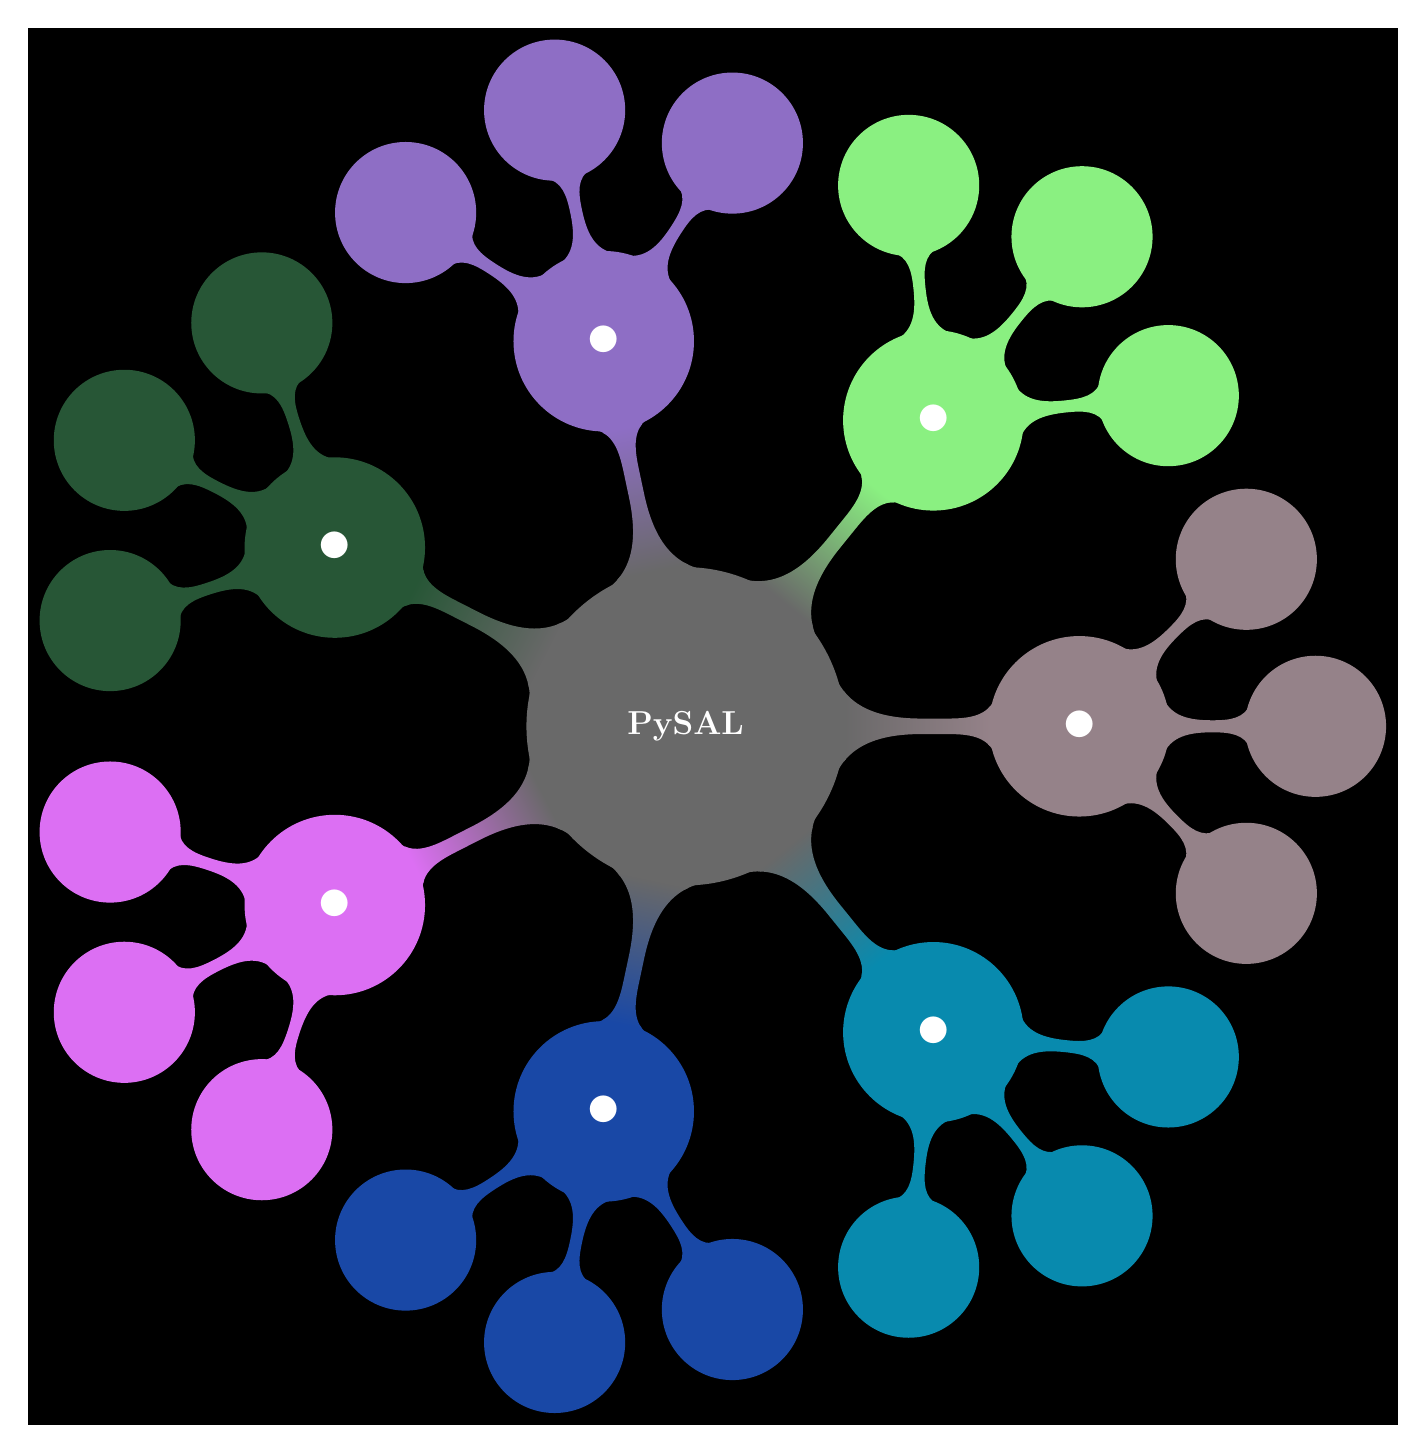
\begin{tikzpicture}[
        background rectangle/.style={fill=black},
        show background rectangle,
        mindmap,
        grow cyclic,
        every node/.style=concept,
        concept color=dimgray,
        text=white,
        level 1/.append style={
            level distance=5cm,
            sibling angle=51,
            font=\Huge
        },
        level 2/.append style={
            level distance=3cm,
            sibling angle=45
        }
    ]
    
        \node[concept color=dimgray]{\large\bfseries{PySAL}}
        child [concept color=220_111_243]{ node {$\bullet$}
            child { node { }}
            child { node { }}
            child { node { }}
         }
        child [concept color=25_72_166]{ node {$\bullet$}
            child { node { }}
            child { node { }}
            child { node { }}
         }
        child [concept color=8_138_174]{ node {$\bullet$}
            child { node { }}
            child { node { }}
            child { node { }}
         }
        child [concept color=149_130_137]{ node {$\bullet$}
            child { node { }}
            child { node { }}
            child { node { }}
         }
        child [concept color=138_240_129]{ node {$\bullet$}
            child { node { }}
            child { node { }}
            child { node { }}
         }
        child [concept color=142_110_197]{ node {$\bullet$}
            child { node { }}
            child { node { }}
            child { node { }}
         }
        child [concept color=39_86_54]{ node {$\bullet$}
            child { node { }}
            child { node { }}
            child { node { }}
         }
                ;
    \end{tikzpicture}
    \end{document}